\section{Circuit Diagram}
\markright{Circuit Diagram}

In this experiment, we construct a full-wave bridge rectifier circuit connected to a center-tapped transformer with a 12V secondary winding. The circuit consists of four silicon diodes (1N4007) arranged in a bridge configuration with a load resistor and optional filter capacitor.

\begin{figure}[H]
  \centering
  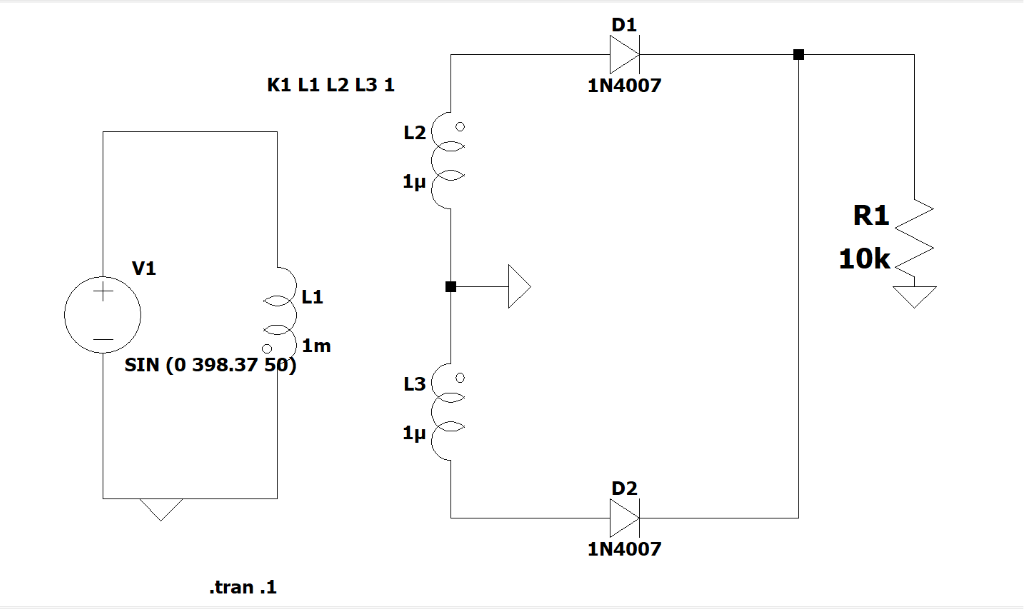
\includegraphics[width=0.7\textwidth]{lab-04/assets/center-tapped-without-capacitor-schematic.png}
  \caption{Experimental circuit diagram showing the full-wave bridge rectifier with a 12V center-tapped transformer, four silicon diodes, a 10\,k$\Omega$ load resistor ($R_L$), and a 10\,$\mu$F filter capacitor. The oscilloscope is connected to measure both input and output voltages.}
  \label{fig:circuit_diagram_lab04}
\end{figure}

The center-tapped transformer provides a dual secondary output with opposite phases. The four diodes are connected such that during each half-cycle of the AC input, two diodes conduct in series through the load, ensuring that current always flows in the same direction through $R_L$. When the optional filter capacitor is connected in parallel with the load resistor, it charges during the diode conduction periods and discharges through the load during non-conduction periods, thereby smoothing the output voltage and reducing ripple.
